%!TEX program = xelatex
% This is a small sample LaTeX input file (Version of 10 April 1994)
%
% Use this file as a model for making your own LaTeX input file.
% Everything to the right of a  %  is a remark to you and is ignored by LaTeX.
 
% The Local Guide tells how to run LaTeX.
 
% WARNING!  Do not type any of the following 10 characters except as directed:
%                &   $   #   %   _   {   }   ^   ~   \   
 
%\documentclass{article}        % Your input file must contain these two lines 
\documentclass[12pt, a4paper, oneside]{ctexart}
\usepackage{xeCJK}

\usepackage{indentfirst, abstract, appendix} %首行缩进
\usepackage{graphicx} %插入图片
\usepackage{amsmath, amssymb, geometry} 
\usepackage{listings, xcolor} %代码高亮
\graphicspath{{../graphics/}}
\linespread{1.2}
\geometry{left=2.5cm, right=2.5cm, top=2.5cm, bottom=2.5cm}
\title{\textbf{SVM的数学推导和Python实现}}
\author{赵新锋}
\date{\today}
\renewcommand{\abstractname}{\Large\textbf{摘要}}
\pagestyle{plain}

\lstset{ %
language=Python,                % the language of the code
basicstyle=\footnotesize,           % the size of the fonts that are used for the code
%numbers=left,                   % where to put the line-numbers
%numberstyle=\tiny\color{gray},  % the style that is used for the line-numbers
stepnumber=2,                   % the step between two line-numbers. If it's 1, each line 
                                % will be numbered
numbersep=5pt,                  % how far the line-numbers are from the code
backgroundcolor=\color{white},      % choose the background color. You must add \usepackage{color}
showspaces=false,               % show spaces adding particular underscores
showstringspaces=false,         % underline spaces within strings
showtabs=false,                 % show tabs within strings adding particular underscores
frame=single,                   % adds a frame around the code
rulecolor=\color{black},        % if not set, the frame-color may be changed on line-breaks within not-black text (e.g. commens (green here))
tabsize=2,                      % sets default tabsize to 2 spaces
captionpos=b,                   % sets the caption-position to bottom
breaklines=true,                % sets automatic line breaking
breakatwhitespace=false,        % sets if automatic breaks should only happen at whitespace
title=\lstname,                 % show the filename of files included with \lstinputlisting;
                                % also try caption instead of title
keywordstyle=\color{blue},          % keyword style
commentstyle=\it\color[RGB]{0,96,96},                % 设置代码注释的格式
stringstyle=\rmfamily\slshape\color[RGB]{128,0,0},         % string literal style
escapeinside={\%*}{*)},            % if you want to add LaTeX within your code
morekeywords={*,...}               % if you want to add more keywords to the set
}
\begin{document}               % plus the \end{document} command at the end.
\maketitle

\setcounter{page}{0}
\maketitle
\thispagestyle{empty}

\begin{abstract}
支持向量机(support vector machines, SVM)是一种分类模型,该模型在特征空间中求解间隔最大的分类超平面。
\par\textbf{关键词:}支持向量机; SVM; SMO; 矩阵运算; 矩阵求导;numpy;sklearn. 
\end{abstract}

\newpage
\pagenumbering{Roman}
\setcounter{page}{1}
\tableofcontents
\newpage
\setcounter{page}{1}
\pagenumbering{arabic}


\newpage
\section{数学推导与python实现}

\subsection{分类超平面}
简单说明如下:
\begin{figure}[htbp]
    \centering
    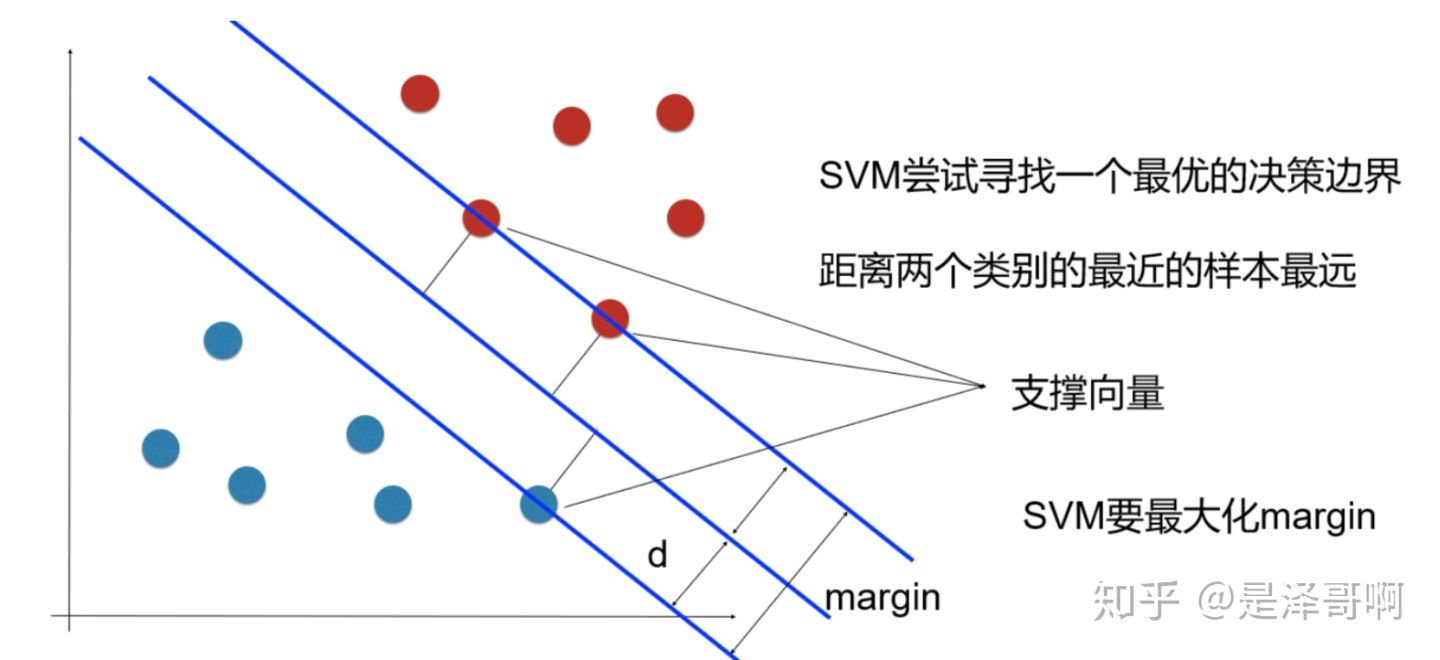
\includegraphics[width=14cm]{svm1.jpg}
    \caption{SVM线性可分}\label{fig1}
\end{figure}



\subsection{公式推导}
过程表示如下:    
\begin{align}
    \mathop{\arg\max}_{w_0} \ d &= \frac{y_0 \cdot (x_0^T \cdot w_0 + b_0)}{ \left\|w_0\right\|} 			\label{eq1}\\
	\mathrm{ s.t. }\ \   &\frac{y_i \cdot (x_i^T \cdot w_0 + b_0)}{ \left\|w_0\right\|} \geq d				\nonumber
\end{align}
将 $w_0$ 和 $b_0$ 进行一定比例的缩放
\begin{align}
	w &= \frac{w_0 }{ y_0 \cdot (x_0^T \cdot w_0 + b_0)} 			\nonumber\\
    b &= \frac{b_0 }{ y_0 \cdot (x_0^T \cdot w_0 + b_0)} 			\nonumber
\end{align}
可以将 \eqref{eq1} 式化简为:
\begin{align}
	\mathop{\arg\max}_{w} \ d &= \frac{1}{ \left\|w\right\|} 			\nonumber\\
    \iff \mathop{\arg\min}_{w}  \ d &=  \left\|w\right\| \nonumber\\
    \iff \mathop{\arg\min}_{w}  \ d &=  \frac{1}{2}w^T \cdot w \label{eq2}\\
    \mathrm{ s.t. }\ \   & y_i \cdot (x_i^T \cdot w + b) \geq 1				\label{eq3}
\end{align}
将\eqref{eq2} 和 \eqref{eq3} 利用拉格朗日乘数法,获得拉格朗日原始问题形式:
\begin{align}
    \mathop{\arg\min_{w,b}\max_{\alpha}} \ 	L(w, b, {\alpha}) &= \frac{1}{2}	w^T \cdot w  - {\alpha} ^T \cdot  (y \odot (X \cdot w + b) - 1) \nonumber\\
        &= \frac{1}{2}	w^T \cdot w  - (\alpha \odot y) ^T \cdot  (X \cdot w + b) - \alpha^T \cdot \boldsymbol{1}^m \nonumber\\
        &= \frac{1}{2}	w^T \cdot w  - (\alpha \odot y) ^T \cdot  (X \cdot w + b) - \boldsymbol{1}^T\cdot\alpha \label{eq4}
\end{align}
当满足KTT条件时, \eqref{eq4} 等价于拉格朗日对偶问题:
\begin{align}
    \mathop{\arg\max_{\alpha}\min_{w,b}} \ 	L(w, b, {\alpha}) &= \frac{1}{2}	w^T \cdot w  - (\alpha \odot y) ^T \cdot  (X \cdot w + b) - \boldsymbol{1}^T\cdot\alpha \label{eq4_1}
\end{align}
首先求L以 w、b为参数的极小值,通过求微分得到偏导数形式。
\begin{align}
    \mathrm{d}L &= \frac{1}{2}tr[(\mathrm{d}w)^T \cdot w + w^T \cdot \mathrm{d}w) - (\alpha \odot y) ^T \cdot(X\mathrm{d}w) \nonumber \\
                & \ \ \  - (\alpha \odot y) ^T \cdot \mathrm{d}b \nonumber\\
                & \ \ \  - (\mathrm{d}\alpha)^T \cdot (y \odot (X \cdot w + b) - 1)] \nonumber \\
                &= tr[w^T\mathrm{d}w - (X^T\cdot(\alpha \odot y))^T\mathrm{d}w - (\alpha \odot y) ^T \cdot \mathrm{d}b - (y \odot (X \cdot w + b) - 1)^T\mathrm{d}\alpha] \nonumber
\end{align}
从而得到w、b 偏导数,并令偏导数为0。
\begin{align}
    \frac{\partial L}{\partial w} &= w - X^T\cdot(\alpha \odot y) = \boldsymbol{0}\nonumber \\
    \frac{\partial L}{\partial b} &= - \alpha \odot y \nonumber = \boldsymbol{0}\\
\end{align}
推导出如下等式和约束:
\begin{align}
    w &= X^T\cdot(\alpha \odot y) \label{eq6} \\
    \alpha \odot y &= \boldsymbol{0} \label{eq7}
\end{align}
将\eqref{eq6}式 和 \eqref{eq7}式 代入\eqref{eq4_1}式中,
\begin{align}
    \mathop{\arg\max}_{\alpha} L(w, b, {\alpha}) &= \frac{1}{2}(\alpha \odot y)^T \cdot X^T \cdot X \cdot (\alpha \odot y) \nonumber \\
                      & \ \ \  - (\alpha \odot y)^T \cdot X^T \cdot X \cdot (\alpha \odot y) \nonumber \\
                      & \ \ \  - (\alpha \odot y)^T \cdot b^m  \nonumber \\
                      &= -\frac{1}{2}(\alpha \odot y)^T \cdot X^T \cdot X \cdot (\alpha \odot y) + (\alpha \odot y^T) \cdot b \nonumber \\
                      &= -\frac{1}{2}(\alpha \odot y)^T \cdot X^T \cdot X \cdot (\alpha \odot y) \nonumber 
\end{align}
去除符号,将极大转换成极小形式:
\begin{align}
    \mathop{\arg\min}_{\alpha} L(w, b, {\alpha}) &= \frac{1}{2}(\alpha \odot y)^T \cdot X^T \cdot X \cdot (\alpha \odot y) \label{eq9} \\
        \mathrm{ s.t. }\ \   \alpha \odot y &= \boldsymbol{0} \nonumber 
\end{align}
加入软间隔参数,每个向量点距离分类超平面距离增加$\xi_i$,同时增加一个惩罚系数C,代入\eqref{eq4_1}新形式如下:
\begin{figure}[htbp]
    \centering
    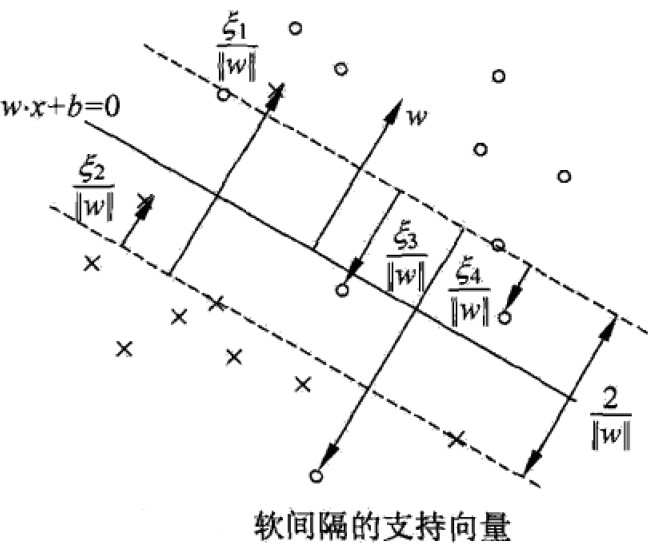
\includegraphics[width=14cm]{svm_soft.jpg}
    \caption{SVM软间隔}\label{fig2}
\end{figure}
\begin{align}
    L(w, b, \xi, {\alpha}, u) &= \frac{1}{2}w^T \cdot w + C \cdot \xi^T \cdot\boldsymbol{1}^m   - {\alpha} ^T \cdot  (y \odot (X \cdot w + b) - 1) - u^T \cdot \xi  \label{eq10} 
\end{align}
求得对于w、b、$\xi$ 的偏导并令其为0:
\begin{align}
    \frac{\partial L}{\partial w} &= w - X^T\cdot(\alpha \odot y) = \boldsymbol{0} \nonumber \\
    \frac{\partial L}{\partial b} &= - \alpha \odot y  = \boldsymbol{0} \nonumber  \\
    \frac{\partial L}{\partial \xi} &= C - \alpha - u  = \boldsymbol{0} \nonumber 
\end{align}
代入 \eqref{eq10} 式中: 
\begin{align}
    \mathop{\arg\max_{\alpha}}  L(w, b, \xi, {\alpha}, u) &= -\frac{1}{2}(\alpha \odot y)^T \cdot X^T \cdot X \cdot (\alpha \odot y) + \boldsymbol{1}^m \cdot \alpha \label{eq11} \\
    \mathrm{ s.t. }\ \   &\alpha \odot y = \boldsymbol{0} \nonumber \\
    &C - \alpha - u \nonumber  = \boldsymbol{0} \nonumber \\
    &\alpha_i \geq 0 \nonumber \\
    &u_i \geq 0 \nonumber 
\end{align}

End!!




\end{document}                 % The input file ends with this command.

